%%%%%%%%%%%%%%%%%%%%%%%%%%%%%%%%%%%%%%%%%%%%%%%%%%%%%%%%%%%%%%
%%%%%%%%%%%%%%%%%%%%%%%%%%%%%%%%%%%%%%%%%%%%%%%%%%%%%%%%%%%%%%
%%                                                          %%
%% Important note on usage                                  %%
%% -----------------------                                  %%
%% This file should normally be compiled with PDFLaTeX      %%
%% Using standard LaTeX should work but may produce clashes %%
%%                                                          %%
%%%%%%%%%%%%%%%%%%%%%%%%%%%%%%%%%%%%%%%%%%%%%%%%%%%%%%%%%%%%%%
%%%%%%%%%%%%%%%%%%%%%%%%%%%%%%%%%%%%%%%%%%%%%%%%%%%%%%%%%%%%%%

%% The '3p' and 'times' class options of elsarticle are used for Elsevier CRC
%% Add the 'procedia' option to approximate to the Word template
%\documentclass[3p,times,procedia]{elsarticle}
\documentclass[3p,times]{elsarticle}

%% The `ecrc' package must be called to make the CRC functionality available
\usepackage{ecrc}

%% The ecrc package defines commands needed for running heads and logos.
%% For running heads, you can set the journal name, the volume, the starting page and the authors

%% set the volume if you know. Otherwise `00'
\volume{00}

%% set the starting page if not 1
\firstpage{1}

%% Give the name of the journal
\journalname{Future Generation Computing Systems}

%% Give the author list to appear in the running head
%% Example \runauth{C.V. Radhakrishnan et al.}
\runauth{L. Miroslaw et al.}

%% The choice of journal logo is determined by the \jid and \jnltitlelogo commands.
%% A user-supplied logo with the name <\jid>logo.pdf will be inserted if present.
%% e.g. if \jid{yspmi} the system will look for a file yspmilogo.pdf
%% Otherwise the content of \jnltitlelogo will be set between horizontal lines as a default logo

%% Give the abbreviation of the Journal.  Contact the journal editorial office if in any doubt
\jid{fgcs}

%% Give a short journal name for the dummy logo (if needed)
\jnltitlelogo{FGCS}

%% Provide the copyright line to appear in the abstract
%% Usage:
%   \CopyrightLine[<text-before-year>]{<year>}{<restt-of-the-copyright-text>}
%   \CopyrightLine[Crown copyright]{2011}{Published by Elsevier Ltd.}
%   \CopyrightLine{2011}{Elsevier Ltd. All rights reserved}
\CopyrightLine{2011}{Published by Elsevier Ltd.}

%% Hereafter the template follows `elsarticle'.
%% For more details see the existing template files elsarticle-template-harv.tex and elsarticle-template-num.tex.

%% Elsevier CRC generally uses a numbered reference style
%% For this, the conventions of elsarticle-template-num.tex should be followed (included below)
%% If using BibTeX, use the style file elsarticle-num.bst

%% End of ecrc-specific commands
%%%%%%%%%%%%%%%%%%%%%%%%%%%%%%%%%%%%%%%%%%%%%%%%%%%%%%%%%%%%%%%%%%%%%%%%%%

%% The amssymb package provides various useful mathematical symbols
\usepackage{amssymb}
\usepackage{url}
%% The amsthm package provides extended theorem environments
%% \usepackage{amsthm}

%% The lineno packages adds line numbers. Start line numbering with
%% \begin{linenumbers}, end it with \end{linenumbers}. Or switch it on
%% for the whole article with \linenumbers after \end{frontmatter}.
%\usepackage{lineno}

%% natbib.sty is loaded by default. However, natbib options can be
%% provided with \biboptions{...} command. Following options are
%% valid:

%%   round  -  round parentheses are used (default)
%%   square -  square brackets are used   [option]
%%   curly  -  curly braces are used      {option}
%%   angle  -  angle brackets are used    <option>
%%   semicolon  -  multiple citations separated by semi-colon
%%   colon  - same as semicolon, an earlier confusion
%%   comma  -  separated by comma
%%   numbers-  selects numerical citations
%%   super  -  numerical citations as superscripts
%%   sort   -  sorts multiple citations according to order in ref. list
%%   sort&compress   -  like sort, but also compresses numerical citations
%%   compress - compresses without sorting
%%
%% \biboptions{comma,round}

% \biboptions{}

% if you have landscape tables
\usepackage[figuresright]{rotating}

% put your own definitions here:
%   \newcommand{\cZ}{\cal{Z}}
%   \newtheorem{def}{Definition}[section]
%   ...

% add words to TeX's hyphenation exception list
%\hyphenation{author another created financial paper re-commend-ed Post-Script}

% declarations for front matter

\usepackage[utf8]{inputenc} % set input encoding (not needed with XeLaTeX)
\usepackage{wrapfig} 
\usepackage{subcaption}
\usepackage{graphicx} % support the \includegraphics command and options

%%% PACKAGES
%\usepackage{booktabs} % for much better looking tables
%\usepackage{tikz}
\usepackage{todonotes}
%\usepackage{array} % for better arrays (eg matrices) in maths
%\usepackage{paralist} % very flexible & customisable lists (eg. enumerate/itemize, etc.)
%\usepackage{verbatim} % adds environment for commenting out blocks of text & for better verbatim
%\usepackage{subfig} % fmake it possible to include more than one captioned figure/table in a single float
% These packages are all incorporated in the memoir class to one degree or another...

%%% SECTION TITLE APPEARANCE
%\usepackage{sectsty}
%\allsectionsfont{\sffamily\mdseries\upshape} % (See the fntguide.pdf for font help)
% (This matches ConTeXt defaults)

%%% ToC (table of contents) APPEARANCE
%\usepackage[nottoc,notlof,notlot]{tocbibind} % Put the bibliography in the ToC
%\usepackage[titles,subfigure]{tocloft} % Alter the style of the Table of Contents
%\renewcommand{\cftsecfont}{\rmfamily\mdseries\upshape}
%\renewcommand{\cftsecpagefont}{\rmfamily\mdseries\upshape} % No bold!

%%% END Article customizations

\DeclareGraphicsExtensions{.pdf,.png,.jpg}
\graphicspath{ {../figs/} }

\begin{document}

\begin{frontmatter}

%% Title, authors and addresses

%% use the tnoteref command within \title for footnotes;
%% use the tnotetext command for the associated footnote;
%% use the fnref command within \author or \address for footnotes;
%% use the fntext command for the associated footnote;
%% use the corref command within \author for corresponding author footnotes;
%% use the cortext command for the associated footnote;
%% use the ead command for the email address,
%% and the form \ead[url] for the home page:
%%
%% \title{Title\tnoteref{label1}}
%% \tnotetext[label1]{}
%% \author{Name\corref{cor1}\fnref{label2}}
%% \ead{email address}
%% \ead[url]{home page}
%% \fntext[label2]{}
%% \cortext[cor1]{}
%% \address{Address\fnref{label3}}
%% \fntext[label3]{}

\dochead{Big Data in the Cloud}
%% Use \dochead if there is an article header, e.g. \dochead{Short communication}
%% \dochead can also be used to include a conference title, if directed by the editors
%% e.g. \dochead{17th International Conference on Dynamical Processes in Excited States of Solids}

\title{Unified cloud orchestration framework for elastic high performance computing in the cloud}
% NAFEMS: A unified framework for orchestration of numerical simulations in the Windows Azure cloud platform

%% use optional labels to link authors explicitly to addresses:
%% \author[label1,label2]{<author name>}
%% \address[label1]{<address>}
%% \address[label2]{<address>}

\author[hsr,pwr]{Lukasz Miroslaw}
\author[eth]{Michael Pantic}
%\author[hsr]{Vladimir Baros}
\author[hsr]{Henrik Nordborg}

\address[hsr]{Institute for Energy Technology, Hochschule Rapperswil, Switzerland}
\address[eth]{ETH Zurich, Switzerland}
\address[pwr]{Wroclaw University of Technology, Poland}

\begin{abstract}
%The efficient use of numerical simulations, such as computational fluid dynamics, requires significant computing power, usually only available through large and expensive cluster systems. This effectively hinders small and medium organizations from simulating, as those clusters need to be sized sufficiently large and highly utilized to be profitable.
%Those problems can be solved using elastic, pay-per-use cloud computing. In this paper, we show how well different problems scale with different machines and cluster configurations within Microsoft Azure. We also focused on decreasing computational time without increasing the total costs of operation, using dynamic, short-term allocation of nodes. Additionally, we give a short introduction on how MPI jobs can be executed with no pre-existing infrastructure. Performance estimates and comparisons with traditional on-site clusters are made using the HPL and HPCG benchmarks.
%\todo[inline]{maybe say something about the goal of lowering the entry barriers for simulating.} 

Numerical simulations stand in need for scalable computing power, storage and high availability that can be provided only through expensive and large clusters. While this is still a preferred option for research institutions, government agencies and large companies, institutions with smaller budget usually can not afford large investments. Apparently, the reasonable return of investment is only possible when the clusters are highly utilized and sized optimally depending on the actual demands. 
Those problems can be solved using elastic, pay-per-use cloud computing platforms. Still, accessing own applications in the cloud is a tedious task and requires a significant amount of effort and expertise in cloud computing. Bringing a specific application to the IaaS infrastructure is difficult to achieve. A numerical application that needs to be deployed is usually a command line-tool that requires a similarly complex deployment steps as on the private cluster, e.g. installation, configuration as well as setting up system specific services and network policies. This can be too cumbersome for a domain engineer or a scientist. A simple mechanism is needed to simplify the whole process and lower the entry barrier for cloud-based simulations.
Therefore, we present a unified framework to submit an application directly to the cloud in a simple way. The platform integrates Microsoft Azure specific HPC libraries with PowerShell commandlets to ease the submission process while keeping the desired command line environment. The framework provides tools with the ability to deploy necessary number of virtual machines dynamically, submit the packed application together with input and configuration files, execute the simulation and, once the results are ready, download them to the local machine and stop the virtual machines. 
We demonstrate our framework in orchestration of two scalable and large simulations in the domain of Computational Fluid Dynamics where the Big Data has always been a concern. In addition, we also show how well selected computational problems scale with different machines and cluster configurations within Microsoft Azure. We also provide performance estimates and comparison with a traditional on-site cluster.


\end{abstract}

\begin{keyword}
microsoft azure \sep high performance computing
%% keywords here, in the form: keyword \sep keyword

%% PACS codes here, in the form: \PACS code \sep code

%% MSC codes here, in the form: \MSC code \sep code
%% or \MSC[2008] code \sep code (2000 is the default)

\end{keyword}

\end{frontmatter}

%\linenumbers 

\section{Introduction} 
\label{sec:introduction}
% why we need CFD in the cloud (Henrik)

Computational fluid dynamics (CFD) and numerical simulations are powerful methods to support engineering designs and reduce development costs in both industry and research. Since Navier-Stokes equations have been formulated in the XIX. century, it became possible to study the motion of viscous fluids and model many physical phenomena of great importance for industry, science and society. For example CFD can be used to model the water flow in a pipe, the development of an electrical arc, blood flow in the human aorta, ocean currents or the air flow around a wing. 

The recent advances in information technology made it possible to analyze larger models with higher precision in shorter time. This requirement calls for large amounts of computational power, which typically is provided by large, expensive on-premise clusters. On the one hand, such systems are unavailable to small or medium enterprises that have limited access to clusters and thus numerical simulations are often not considered as viable alternatives to traditional prototyping. On the other hand, research groups are not capable of solving their models locally, making them dependent on external clusters.

%\todo[inline]{describe existing tools} 
A majority of the advanced CFD solvers are able to run concurrently. They take advantage of the Message Passing Interface Standard \cite{openfoam}, OpenMP or both. There are also solvers that run on hardware accelerators such as General Processing Graphics Processing Units \cite{tomczak2013} or Intel Phi \cite{Che09042015}. "CFX" by ANSYS is a commonly used solver in both industry and research. The company is one of the largest player in the Computer Aided Engineering (CAE) market \cite{mcae2012} and its software is typically used for the largest simulations composed of millions of cells. Big Data in the CAE domain has become a challenge for HPC engineers as it requires larger and larger clusters and only recently, a shift towards cloud-based solution has been observed.

% what is the cloud, what are the problems
Cloud computing has become ubiquitous due to its flexibility and cost-efficiency. It has clear advantages over traditional on-premise systems for institutions with limited budgets as no direct investments are needed and machines can be rented on an hourly basis. Users benefit from the cloud through the possibility of launching jobs of different sizes on dynamically sized systems and the cloud operators achieve economies of scale by building large data centers where the resources can be shared between different workloads. \\
An increasing amount of computing power is now hosted on cloud platforms such as Amazon Elasting Compute (EC2) \cite{ec2}, Cloud Foundry Google Compute Engine \cite{google} or Microsoft Azure \cite{azure} and more and more software and services are being hosted in the cloud. Many independent software vendors (ISV) started to offer cloud services to scale scientific applications for specific industries. Many ISVs like Rescale, Ciespace, Ubercloud, Sabalcore, Univa, Penguin Computing provide cloud services for weather research, computational fluid dynamics, structural mechanics, quantitative finance, combustion, electromagnetics and molecular dynamics \cite{theuebercloud}. They offer access to VMs with preinstalled software or a web portal where the scientific applications, such as ANSYS, Gromacs, OpenFOAM or Gerris solvers can be executed \cite{Popinet2003}.

%of using the cloud is the security. The jobs are executed on a hardware in unknown location that is not fully controlled by the user. The cloud providers do their best to convince the user that the data is saved by using different security policies. 

While this may be a satisfying solution for some, the ability to run custom or third-party software on the cloud infrastructure requires much more complicated procedures. A scientific application that needs to be deployed in the Cloud usually consists of a command line-tool that requires complex deployment steps such as installation, configuration as well as setting up system specific services and network policies, comparable to the effort of administering a on-premises cluster. Access to the deployed applications from a local machine is also a tedious procedure and requires a significant amount of effort. This partly explains why this scenario is often too cumbersome for a domain engineer or a scientist.  

A simple mechanism is needed to simplify the whole process and lower the entry barrier for cloud-based numerical simulations. Such mechanisms exist for Amazon EC2 \cite{ec2} \cite{eucalyptus} but Microsoft Azure still lacks an easy-to-use framework to simplify cloud  orchestration, although it is a platform that is well positioned on the market \cite{Garg2013}.

We present a unified framework, named "SimplyHPC",  that greatly simplifies the use of a distributed application on Microsft Azure. The framework combines Azure specific HPC libraries, deployment tools, machine and MPI configuration into a common platform. Its functionality is, among others, exposed through PowerShell commandlets that ease the submission process while keeping the desired command line environment and flexibility. The framework provides tools with the ability to deploy an arbitrarly number of virtual machines dynamically, submit the packed application together with input and configuration files, execute it as a cloud service using Message Passing Interface (MPI) and, once the results are ready, download them to the local machine and stop the virtual machines. 

Our paper focuses on the following aspects. Chapter \ref{sec:architecture} describes the main components of the proposed framework as well as the platform architecture. Chapter \ref{sec:results} demonstrates the utility of the tool on two scientific applications, namely PETSc and HPCG. In addition we present the scalability study of ANSYS CFX, a commercial fluid dynamics code for realistic, industrial simulations in a Big Data scenario. The paper ends with conclusions and future plans.

%VERY INTERESTING

%	\item[II] We measured how well different applications scale on a cloud computing platform (Microsoft Azure), evaluating feasibility and %cost of operation for different applications and optimizing the machine count / machine size ratio to get as much GFLOPs per \$ as possible.

%\end{itemize}

\section{Background}
\label{sec:background}
\subsection{Motivation}

% there are a few frameworks, not for Azure
Each of the previously mentioned cloud platforms offers different strategies to communicate with the cloud infrastructure and different virtualization procedures. The user is free to manage the cloud resources by deploying the cluster manually or with the help of accompanying scripts and APIs, or use the cloud orchestrators that automate the management of the cloud-based infrastructure. The motivation for our development was twofold.

\begin{description}
\item[Complex deployment] The IaaS cloud requires the user to deploy the application in a similar and often complex way as on the local cluster. Cloud orchestrators manage the interactions and interconnections among cloud-based and on-premises business units as well as expose various automated processes and associated resources. They have become a desired alternative to standard deployment procedures because of lower level of expertise and reduced deployment time. Tools for cloud orchestration and vertical and horizontal scaling are fundamental to the adoption of the framework aiming at simplifying the whole procedure.

\item[Complicated access] Although cloud orchestrators play an important role, still there are only a few easy to use, out-of-the box platforms that simplify deployment, monitoring and accessing scientific applications in the cloud. Companies offering cloud-based software in PaaS model limit their offering to applications of the highest commercial impact while neglecting other types of software such as numerical simulations \cite{CloudStack} \cite{OpenStack}. The best situation is in Amazon EC2 where frameworks to simplify the process of orchestration of specific scientific applications exist. Wong and Goscinski propose a unified framework composed of a series of scripts for running gene sequencing analysis jobs through a web portal \cite{Wong2013} on Amazon EC2 (IaaS) infrastructure. For this purpose they designed a HPC service software library for accessing high level HPC resources from the IaaS cloud and demostrate their framework in running mpiBLAS \cite{mpiBlas}. Balgacem et al. measured the multiphase flow on a hybrid platform combined with Amazon $EC2$ and a private cluster \cite{BenBelgacem2015}. Morpho is a modified version of Hadoop MapReduce framework that decouples storage and computation into physical and virtual clusters to reduce costly data movement of user data \cite{Lu2014}. The authors demonstrate the efficiency of the  framework in text mining application compared with the Hadoop MapReduce running in Amazon mode. Twister4Azure is a MapReduce frameworks designed specifically for Microsoft Azure. It extends the native Hadoop framework in Azure cloud platform and provides multi-level data caching mechanism to overcome the latencies of cloud services as well as a decentralized task scheduling to avoid single point of failure. Still, the framework requires a programming knowledge since it is relased as .NET Project. The platform has been demonstrated in applications that are well fitted to MapReduce paradigm, such as BLAS sequence searching or KMean Clustering. Marozzo et. al \cite{catlett2013cloud} present a web-based framework for running pre-defined workflows composed of web services in Microsoft Azure. The authors demonstrate the framework in data mining applications by deploying an execution workflow running a single classification algorithm and measure strong scalability in classifying different data sets that were previously partitioned. Unfortunately, it is not clear if the algorithm was multi- or single-threaded or if is possible to add own applications to the framework that are no exposed as web-services and not related to data mining. 
Another interesting frameworks are Eucalyptus \cite{eucalyptus} or CloudStack \cite{CloudStack} that were designed to deploy IaaS hybrid clouds, e.g. scalable IaaS cloud computing platform composed of a private cloud and public one based on Amazon EC2.
\end{description}

Due to the fact that the cloud providers are commercial entities that compete on the market, it is hardly impossible to create a single orchestrator that supports the major cloud platforms. The cloud infrastructure changes very quickly, the new APIs, services and tools are released frequently and addressing them in one consistent software is ineffective from a strategical point of view. This is a reason why we preferred to focus on a single provider, namely Microsoft Azure.


%many scientific groups run their scientific code on the cloud
%Since that time many groups attempted to evaluate scientific code on cloud platforms. 

%Windows Azure, a platform offered by Microsoft is a well established platform for high performance computing that 
%\todo[inline]{List more examples} 


%In this paper we focus on th
%Frameworks to simplify the process of orchestration of the scientific applications have also been developed. Wong and Goscinski propose a unified framework that integrates an HPC service library, Amazon EC2 for running mpiBLAST jobs through a web portal \cite{Wong2013}. 
% Their framework exposes 

%TODO: Add more frameworks. 

%Still, there are only a few frameworks that simplify deployment on Windows Azure. 

\subsection{Microsoft Azure}

Microsoft Azure is a cloud computing platform providing three types of VM roles. Web and Worker roles in PaaS model provide a set of predefined cloud services for web applications and scalable applications, respectively. VM roles in IaaS model are just bare machines deployed with a specific OS. The platform is well positioned on the market and is competitive to other cloud providers \cite{cloudScores} \cite{twister4azure} with a large user base and third-party cloud services. As of 2015, ten types of different instances available (see \ref{tab:azureVMs}). Computational costs on Microsoft Azure depend on the number of cores, the type of machine and the time of effective usage. The time of effective usage is the time between set-up of the virtual machine and its tear-down, regardless of the actual usage or workload. \\
A8 and A9 are special Azure VM instances which include Infiniband network stack with low latency and Remote Direct Memory Access (RDMA) enabled. Unfortunately, the specification of the CPUs is provided only for these instances, for other VMs only the number of cores, RAM and disk size is provided. There is also a special D-series virtual machines available with solid state drives and slightly faster processors.
 
%TODO: extend the list

	\begin{center}
	\begin{table}
				\begin{tabular}{|c|c|c|c|c|c|}
			\hline
			Instance & Cores & RAM     & Disk size & CPU & Price                    \\ \hline
				A0     & 1     & 0.75 GB & 20 GB      & - & \$0.02/hr (\~\$13/mo)    \\ \hline
				A1     & 1     & 1.75 GB & 70 GB      & - & \$0.08/hr (\~\$57/mo)    \\ \hline
				A2     & 2     & 3.5 GB  & 135 GB     & - & \$0.15/hr (\~\$115/mo)   \\ \hline
				A3     & 4     & 7 GB    & 285 GB     & - & \$0.30/hr (\~\$229/mo)   \\ \hline
				A4     & 8     & 14 GB   & 605 GB     & - & \$0.72/hr (\~\$536/mo)   \\ \hline
				A5     & 2     & 14 GB   & 135 GB     & - & \$0.33/hr (\~\$246/mo)   \\ \hline
				A6     & 4     & 28 GB   & 285 GB     & - & \$0.66/hr (\~\$491/mo)   \\ \hline
				A7     & 8     & 56 GB   & 605 GB     & - & \$1.32/hr (\~\$982/mo)  \\ \hline
				A8     & 8     & 56 GB   & 382 GB     & Intel Xeon E5-2670 & \$2.45/hr (\~\$1,823/mo) \\ \hline
				A9     & 16    & 112 GB  & 382 GB     & Intel Xeon E5-2670 & \$4.90/hr (\~\$3,646/mo) \\ \hline
				A10    & 8     & 56 GB   & 382 GB     & Intel Xeon E5-2670 & \$1.64/hr (\~\$1,220/mo) \\ \hline
				A11    & 16    & 112 GB  & 382 GB     & Intel Xeon E5-2670 & \$3.04/hr (\~\$2,262/mo) \\ \hline
			\end{tabular}
			\label{tab:azureVMs}
			\caption{Microsoft Azure VM instances. Price list retrieved in May $2015$.}
	\end{table}
\end{center}
 

Cloud computing platform provides various services depending on the level of control and complexity that the user accepts. IaaS (Infrastructure as a Service) model exposes Virtual Machines with a predefined operating system (OS) and preinstalled software. After accessing the machine with SSH protocol or Remote Desktop Controller, the user is responsible for system maintenance and software installations. PaaS (Platform as a Service) architecture is exposed as light-weight virtual machines, called {\it Cloud Services}. They are much simpler to use: instead of configuring the Virtual machines the user uploads a packaged application together with the configuration files. This ''deployment package'' is then installed on a fresh virtual machine automatically and exposes its features to the user in a seamless way. If there are any configuration changes the cloud service is removed and reinstalled on the virtual machine together with the updated deployment package. Such a procedure takes usually a few minutes and is  attractive in terms of rental costs of the cloud because the created VM is immediately deleted after usage. \\
Microsoft Azure provides both types of services for different types of applications. IaaS are provided for non-standard, user-defined applications while the PaaS offers easy access to mostly used services such as web servers, applications server or message brokers. Separate entities provide infrastructure for highly available and scalable data storage. Microsoft Azure exposes four storage types to store, manage and control data in the cloud: Blob, Table, Queue and File. Each storage type is able to host different types of data of arbitrary sizes, namely binary files of any type, structured datasets, messages and shared files, respectively. We decided to take advantage of the cloud service (PaaS) to simplify the orchestration procedure and use Blob and Table storage entities for data management. 

\subsection{HPC Pack}

HPC Pack is a framework developed by Microsoft for monitoring, executing and running jobs in both premise and on Azure platform. It contains a set of deployment, monitoring, administration and job scheduling tools for running HPC applications. Originally it was created for Windows HPC clusters composed of dedicated on-premise compute nodes and workstation computers and the support for Microsoft Azure has been added on top of that. HPC Pack exposes functionality that is typical for cluster management software such as deployment of clusters with different configurations, scheduler that maximizes an utilization of the cluster based on priorities, policies and usage patterns and a batch system for submission of multiple short and long running jobs with different amount of resources. The framework also allows for deployment of hybrid clouds, for example to deploy a head node on-premise and control Azure PaaS nodes or to deploy the head node as a IaaS VM and control PaaS VMs from the local machine. It is a recommended framework to control the Azure cloud.

\subsection{Numerical Software}
\label{sec:numerical}

Sparse linear algebra inspired the use cases presented in this study. Large sparse matrices are generated during the discretization of partial differential equations and often appear in scientific or engineering applications. We have selected two scientific software tools, namely PETSc and High Performance Conjugate Gradient (HPCG) Benchmark to demonstrate the utility of our framework, to measure the performance on both Microsoft Azure and local cluster. 
The High Performance Conjugate Gradient \(HPCG\) Benchmark \cite{Heroux2013} is a benchmark program that solves a sparse linear system during discretization of a three-dimensional heat diffusion problem on a semi-regular grid. Domain decomposition with an additive Schwarz preconditioned conjugate gradient method is used to solve the problem where each subdomain is preconditioned using a symmetric Gauss-Seidel sweep. This benchmark is much more relevant than the LINPACK benchmark that is currently used by $Top500$ which is a solver of a dense system of linear equations. As such LINPACK favors computers with very high floating-point computations an streaming memory systems. Colaesed access to memory is easier to achieve when matrix-matrix multiplications and similar operations are performed on dense matrices. While this is a case for many scientific problems, the LINPACK does not adequately expressed the performance of applications that are based on different memory access patterns, in particular the ones stemming from finite volume of finite element methods. HPCG, as more representative, has been used to benchmark the largest clusters such as Tianhe-2 \cite{Xianyi2014} has started to become more popular in definition of Top500 list. It provides a simple way to measure the performance on easy-to-scale case in MFLOPS across multi-node mode. \\
PETSc is a library with a set of nonlinear and Krylov-subspaces linear solvers with the possibility to run external direct solvers as well as GPU-based kernels. Krylov space methods are considered to be as one of ten most important classes of numerical methods and large sparse matrix eigenvalue problems are present in most scientific computing applications \cite{Gutknecht2005}. This is one the reasons why this software is wide used in multiple scientific disciplines such as acoustics, aerodynamics, computational fluid dynamics, combustion and ocean dynamics just to name a few \cite{petsc-efficient}.\\
In addition to the numerical tools, we have selected ANSYS CFX, a high performance fluid dynamic software that is well recognized in industry and has been successfully applied to different fluid flow problems. It simulates many fluid phenomena including steady-state, transient flows of both laminar and turbulent nature as well as multiphase flows, heat transfer and radiation. Since the installation folder must be accessible by all compute nodes, we additionally created a storage file service which provides the installation files to the compute nodes. During the deployment of the compute nodes, the ANSYS CFX installation folder is being mounted on all machines, using the same drive letter. Once ANSYS CFX is accessible by all compute nodes, other preparation steps such as the installation of MPI and SPMD can be scripted with our framework. We will show the corresponding performance studies for large simulations in Chapter \ref{sec:results}.

\section{SimplyHPC Architecture}
\label{sec:architecture}
In this chapter, three main architectural aspects of SimplyHPC are presented. First, the system architecture is explained in terms of the software stack, cluster settings, communication setup and Azure-specific components visible to a single node. Second, we discuss also the structure of the SimplyHPC framework on the cluster level and explain how the software automatizes the setup of nodes and clusters using the given system architecture. Third, the inner software architecture is briefly presented.

\subsection{Node architecture}

As implied in Sec.~\ref{sec:background} there are different type of machines available on Microsoft Azure. Here, PaaS VMs in \textit{Worker Roles} are used, as they have various advantages over traditional virtual machines, especially in terms of manageability and scalability. They also helped to automatize the deployment step. Instead of configuring a machine and setting up software manually as on regular virtual machines, PaaS VMs are set up using a \textit{Deployment Package}. This package contains the machine-specific configuration such as  network adapters, local storage partitions, etc. 

% Network adapters?
% Explain what is the Azure Fabric Controller, what is the difference compared to the Azure Framework
% SimplyHPC Role DLL -> SimplyHPC DLL
% Azure Virtual Drive -> Azure File Storage

The deployment package contains also the components of the software that is about to be executed on the cluster.
New PaaS VMs are then deployed by supplying this deployment package to the Azure Fabric Controller.

In Fig.~\ref{fig:schemaRole}, the schematic architecture of a single node is shown. The particular components are execute in the predefined order as follows. Here, we present the execution sequence for a typical MPI job:

\begin{enumerate}
	\item During the set up phase of the PaaS VM, the deployment package is installed and set up by the Azure Fabric Controller. Some components are configured as a Windows Service in the ''MPI Context''. This context is set up identically on each node and is used for authentication between nodes during the execution of a distributed MPI job.

	\item After the set up phase has finished, the job scheduler inside the SimplyHPC Role DLL is executed by the Azure Framework. This scheduler periodically checks for new jobs in the configured Azure Table/Blob storage. If such a new job is found, it is downloaded to the local storage and executed according to its parameters. Because the MPI execution takes place in another user context, the start of the process is off-loaded to the MPIWrapper Service with the help of inter-process communication via Windows Communication Foundation pipes.

	\item MPIWrapper that is a custom .NET Windows Service starts the application that we want to execute on the cluster and that is configured in the job definition. The application can be any executable, such PETSc, ANSYS CFX, mpiexec job, etc. Because the application runs inside the MPI Context, it has full access to all other nodes using MPI. MPIWrapper also tracks the execution of the process and reports results back to the SimplyHPC Role DLL.

	\item Infrastructure needed to run MPI jobs is composed of SMPD (''Simple Multi-Purpose Daemon'') and Microsoft MPI (MSMPI). They are installed on each node and are used for running parallel and distributed jobs in the Microsoft cluster. MSMPI is the MPI implementation of Microsoft that is able to use fast interconnects such as Infiniband.
\end{enumerate}

\begin{figure}[h]
	\centering
	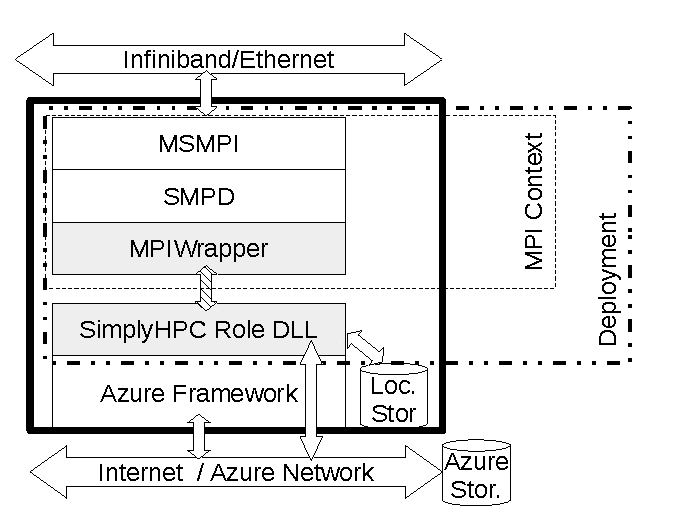
\includegraphics[width=.5\linewidth]{azureWorkerRole.pdf}
	\caption{Schematic view of a single compute node on Azure}

	\label{fig:schemaRole}
\end{figure}

It is important to note that this node architecture applies to all nodes in a cluster, and is automatically configured using the aforementioned deployment package. 


\subsection{Cluster architecture}

Fig.~\ref{fig:schemaService} visualizes all relevant components of a deployed HPC cluster that has been set up using the SimplyHPC framework. 
A \textit{cloud service} (dashed rectangle in figure) is a bundle of multiple nodes using the same deployment template. Using the logical entity of a cloud service, nodes can be easily configured in terms of their number, size and the virtual network they belong to. If autoscaling (?) is needed it can be easily implemented by increasing the number of nodes in the cloud service configuration. If the nodes are overloaded the Azure Fabric Controller will automatically create a new node and applies the deployment template to it.

When using A8/A9 nodes for scientific computing, the internode network (depicted as the upper arrow in Fig.~\ref{fig:schemaService}) is realized with Infiniband. In this mode all internode storage and MPI requests are transparently redirected to this very low latency, high bandwidth interconnect. Such configuration is crucial when best possible scaling is required.

The availability of fast internode connections strongly influences the choice of storage for different tasks. In total, there are four storage types in use and all of them are used within SimplyHPC:

\begin{itemize}

	\item \textit{Azure Table Storage} is a schemaless database accessible by HTTP/REST. SimplyHPC takes advantage of table storage to store configuration information, node synchronization data and job meta data. This table is accessible by all the nodes and can be read by the head node (Arrow 'A' in Fig.~\ref{fig:schemaService}).
	
	\item \textit{Azure Blob Storage} is a storage service used to store large data blocks and accessible by HTTP/REST. Job data such as geometry, matrices, etc. are uploaded from a client to the Azure Blob Storage, and are then copied to the much faster local storage by the head node (Arrow 'B' in Figure \ref{fig:schemaService}). Job results are also uploaded back to this storage and thus made available via internet.	
	
	\item \textit{Azure File Storage} provides a storage which is mountable as a network drive in Windows, and is here used to make software packages available to the worker roles. Large software suites such as ANSYS cannot be included into deployment packages due to its size and can therefore not be directly installed on the PaaS worker roles. Here we used a prepared ANSYS installation on a shared network drive.
	
	\item \textit{Local Storage} is used during job execution for job data (Arrows 'C' in Fig.~\ref{fig:schemaService}). Local storage is realised using local SSD drives an can be shared between nodes using SMBv3 Protocol and Infiniband. Local Storage is the fastest storage available currently on Microsoft Azure. It is important to note that the local storage is not persistent, the data stored get lost after a node has been recreated, restored or updated. Also, local storage is not directly accessible outside the cloud service.

\end{itemize}


\begin{figure}[ht]
	\centering
	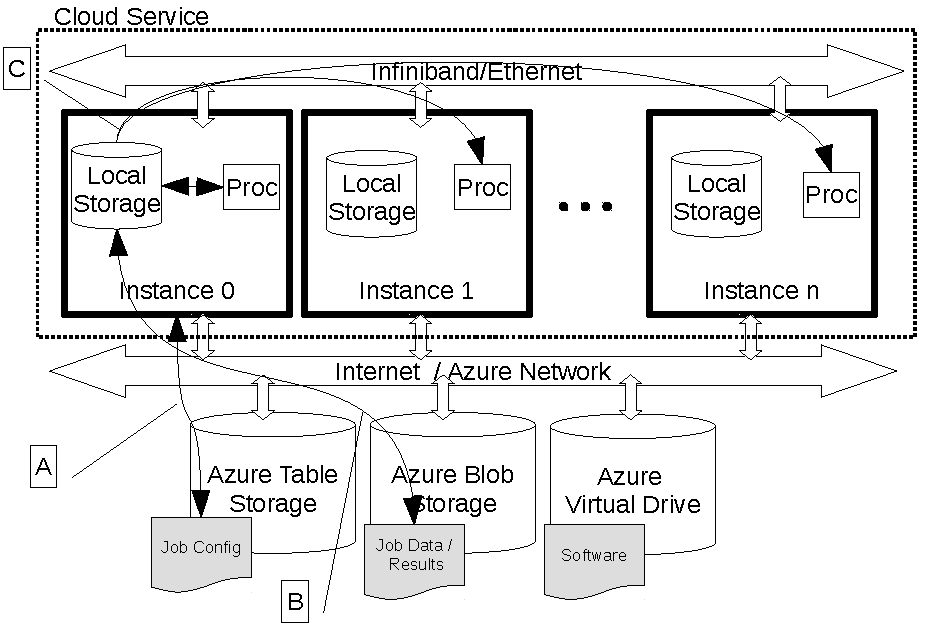
\includegraphics[width=.6\linewidth]{azureDeployment.pdf}

	\caption{Schematic view of a SimplyHPC Cluster on Azure}	
	\label{fig:schemaService}
\end{figure}

\subsection{Software architecture}

SimplyHPC has been written in Visual .NET in /C\# and takes in the advantage C\# and latest Azure mechanisms that automatize the process of setting up of the cluster that we described before. There are multiple levels, at which the SimplyHPC interferes with Microsoft Azure. On the Microsoft Visual SDK Level our framework is integrated in into the Microsoft Azure SDK in order to automatically compile the deployment packages. On the Cloud API Level, SimplyHPC takes advantage of the Azure Cloud Controller to automatize the creation of cloud services, uploading the  deployment packages, monitoring the statuses of the nodes, etc. Finally, on the Azure Framework level, access to the Azure storage, Worker Role startup points was possible and information information about the execution environment could be easily accessed.\\
We expose two different front ends to the user, namely PowerShell commandlets and a high-level API with a facade that hides all the complexity of orchestrating the cloud. 

\begin{table}
	\centering		
		\begin{tabular}{|l|l|}
		\hline
      \textbf{Commandlet} & \textbf{Description} \\ \hline
      NewAzureService & Create a new cloud service and the cluster \\ \hline
			NewAzureJob & Create and execute a new job \\ \hline
			NewAzureParameters & Create a set of parameters required by other commandlets    \\ \hline
			GetJobStatus & Get the status of a given job    \\ \hline
			GetJobResults & Get the results of a given job  \\ \hline
			GetAvailableRoleSizes & Get Available VMs with their roles and sizes \\ \hline
			RemoveAzureJobs & Remove Azure Jobs such as unfinished jobs \\ \hline
			RemoveAzureService & Remove the cloud service and destroy the cluster \\ \hline
    \end{tabular}
	\caption{Commandlets of SimplyHPC framework.}
	\label{tab:CommandletsOfSimplyHPC}
\end{table}

The commandlets are PowerShell modules executed in a specific order and realize specific tasks needed to deploy a scientific application in the cloud, execute it, download the results back to the user and destroy the cluster (see Tab~\ref{tab:CommandletsOfSimplyHPC}).  

\textcolor[rgb]{1,0,0}{API Example and a drawing will help to understand the potential of SimplyHPC.}

\section{Results}
\label{sec:results}
	
The tests were performed in Microsoft Azure cloud from the same subscription as well as in the private cluster. HSR Cluster is a privately owned and maintained cluster at Microsoft Innovation Center at University of Applied Sciences at Rapperswil (HSR), Switzerland. It is composed of $32$ nodes with 48GB RAM and two Intel Xeon E5645 6 cores each, the nodes are connected with 40Gbit Infiniband Network. On each Windows Server $2012$ R2 with HPC Pack 2012 R2. Microsoft provides description of the A8 and A9 nodes only. During the tests we used a cluster with multiple A8 and ExtraLarge instances.

\begin{figure}
\centering
\begin{subfigure}{.5\textwidth}
  \centering
	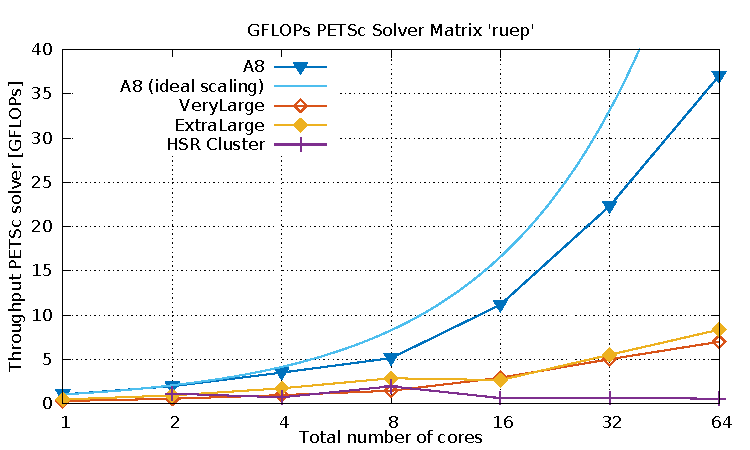
\includegraphics[width=\linewidth]{gplt-gflops-ruep}  
  %\caption{A subfigure}
  \label{fig:ruepel}
\end{subfigure}%
\begin{subfigure}{.5\textwidth}
  \centering
  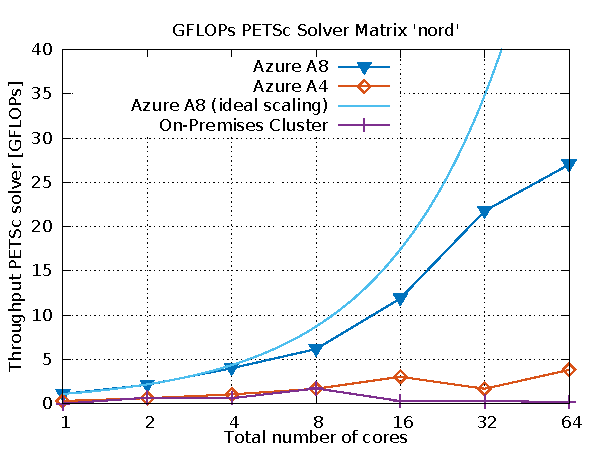
\includegraphics[width=\linewidth]{gplt-gflops-nord}
  %\caption{A subfigure}
  \label{fig:nord}
\end{subfigure}
\caption{Performance in GFlops of PETSc solving ruep (left) and nord (right) matrix systems on different Microsoft Azure nodes and a private HSR cluster. }
\label{fig:test}
\end{figure}

 
First objective was to compare deployment time of a cluster with different number of nodes in both systems. This time should be of the same order regardless the type of role instances because the deployment processes are similar, therefore we performed the tests with a one type of the role instances, namely A4 (see Tab.\ref{tab:azureVMs}). HPC Pack provides a precise statistics on the deployment procedure seperated into individual processes, namely creating a storage account, a virtual network, a cloud service, a domain controller as well as  deployment and configuration time for the head node and compute nodes. Since in SimplyHPC most of these processes were omitted, only the time to deploy the head node and compute nodes was measured, e.g. the time needed to run \textit{NewAzureService} and \textit{NewAzureJob} scripts. Since HPC Pack neither provides automatic job submission nor does it retrieve the result we have not taken these processes into account in our measurements. 

%we measured the time needed create a cluster was measured together with other tasks, i.e. a time needed to pack and send the job to the cluster before the job starts executing.  

\begin{figure}
\centering

  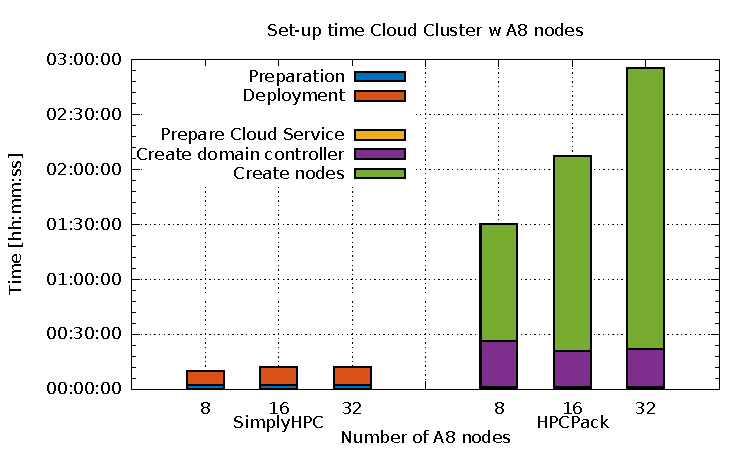
\includegraphics[width=.6\linewidth]{gplt-creation-simplyvshpc}


\caption{Deployment time of cluster composed of different number of A4 nodes with Microsoft HPC pack (right) and SimplyHPC framework (left). Time is provided in hh:mm:ss format.}
\label{fig:deployTime}
\end{figure}

Fig. \ref{fig:deployTime} shows the HPC Pack needs almost an hour to deploy the cluster while the SimplyHPC platform needs about six minutes in average. Such long deployment time lies in the fact HPC Pack performs also additional deployment steps such as creating a domain controller, SQL database or installing many additional services that are not needed for command-line scientific applications.

The objective of the second experiment was to compare the performance of Microsoft Azure with a private cluster by running sparse matrix solver called PETSc. PETSc was run with two matrices: \textit{ruep} and \textit{nord}. The first one comes from thermal transient heat conduction simulation of electrical cabinet on a large unstructured mesh composed of 2.3 millions cells and the second matrix was generated from a thermal transient heat conduction simulation on a 3-dimensional Cartesian mesh of moderate size. Due to different mesh types, the second matrix converges much quicker than the first one. 

\begin{figure}
	\centering
	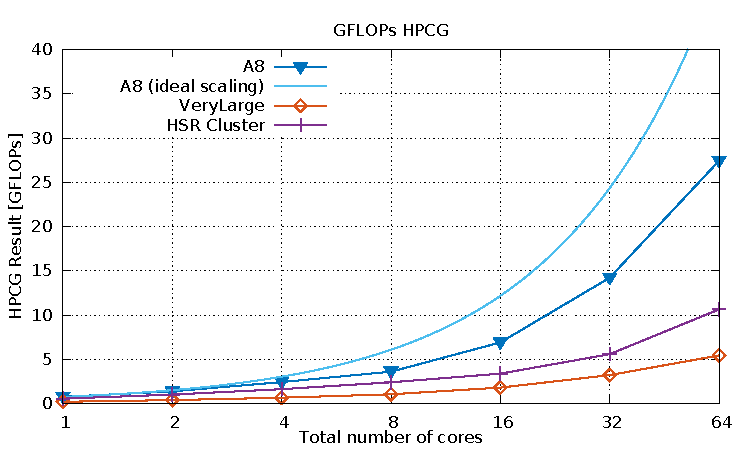
\includegraphics[width=.5\linewidth]{gplt-gflops-hpcg}
	
	\caption{Performance in GFlops of HPCG benchmark on different Microsoft Azure nodes and a private HSR cluster. }
	\label{fig:hpcg}
\end{figure}

Since iterative solvers are memory-bound algorithms we measured the performance achieved for different combinations of cores in a single node, e.g. one node with one, two, four and eight cores and for two, four and eight nodes with eight cores. This way both vertical scaling (adding more cores to the system) and horizontal scaling (adding more nodes to the system) could be approximately measured. %More exact measurements were not executed because the private clusters had different hardware, the objective of the paper is different

HPCG benchmark test confirms the performance achieved on Azure nodes, although a slightly better performance was achieved for the HSR cluster due to suboptimal choice of the number of cores per node.  To illustrate this we run PETSc on HSR cluster with two, four and eight nodes with a single core. For ruep matrix the performance achieved was $2.1$, $4.1$ and $8.1$ GFLOPs, respectively. HPCG benchmark aims at solving a large sparse system of equation derived from a single degree of freedom heat diffusion model with zero Dirichlet boundary conditions. The global domain dimensions were $(nx * npx ) * (ny * npy ) * (nxz * npz )$ where $(nx * ny * nz )$ are the local subgrid dimension in the $x$, $y$, and $z$ dimensions, respectively, assigned to each MPI process. For the study $nx = ny = nz = 240$ and $npx, npy, npz$ are a factoring of the MPI process space that is computed automatically in the HPCG setup phase.

In terms of realistic and large physical simulations we have simulated a heat transfer in the heat exchange system and the fluid flow in a compressor used in the turbines. The heat exchange system is composed of the  pipe where the water flows with the speed of $0.05 m/s$ that is buried in the ground and heated by from external source with the temperature of $10 ^\circ C$ and the heat transfer to the flowing water is simulated. Such a system is used to optimize the energy costs in buildings through the energy reuse.  
Compressors generate air pressure that is critical in a wide range of applications - from corner gas stations to manufacturing and power plants. In our model the air gets to the compressor through a filtered intake that removes the contaminants at the speed of $2.83\ m/s$ at $9.85 ^\circ C$. It then enters the space with three rotors where the air is compressed. Geometries of both systems are presented in Fig.~\ref{fig:cfx}. The size of the first mesh can be scaled  in x-direction due to symmetrical geometry while the size of the compressor has ca. 13 millions cells (see Tab~\ref{tab:MeshSize}). In both cases we modeled the steady state flows with residual targets of $1e\-06$ and $1e\-08$ and maximal number of iterations of $100$ and $200$, respectively. 

\begin{table}
	\centering
		\begin{tabular} {|c|c|c|}
			\hline
			Name & No. of Elements & No. of nodes \\			
			pipe01 & 195'102 & 255'462 \\ \hline
			pipe02 & 432'919 & 512'212 \\ \hline
			pipe06 & 1'017'573 & 1'148'856 \\ \hline
			pipe04 & 2'037'710 & 2'213'036 \\ \hline
			pipe05 & 4'010'210 & 4'313'036 \\ \hline			
			pipe07 & 8'101'299 & 8'526'790 \\ \hline
			pipe08 & 15'522'778 & 16'157'192 \\ \hline
			compressor & 13'799'389  & 11'025'383 \\ \hline
		\end{tabular}
	\caption{The mesh size of test cases}
	\label{tab:MeshSize}
\end{table}

\begin{figure}
\centering
\begin{subfigure}{.4\textwidth}
	\centering
	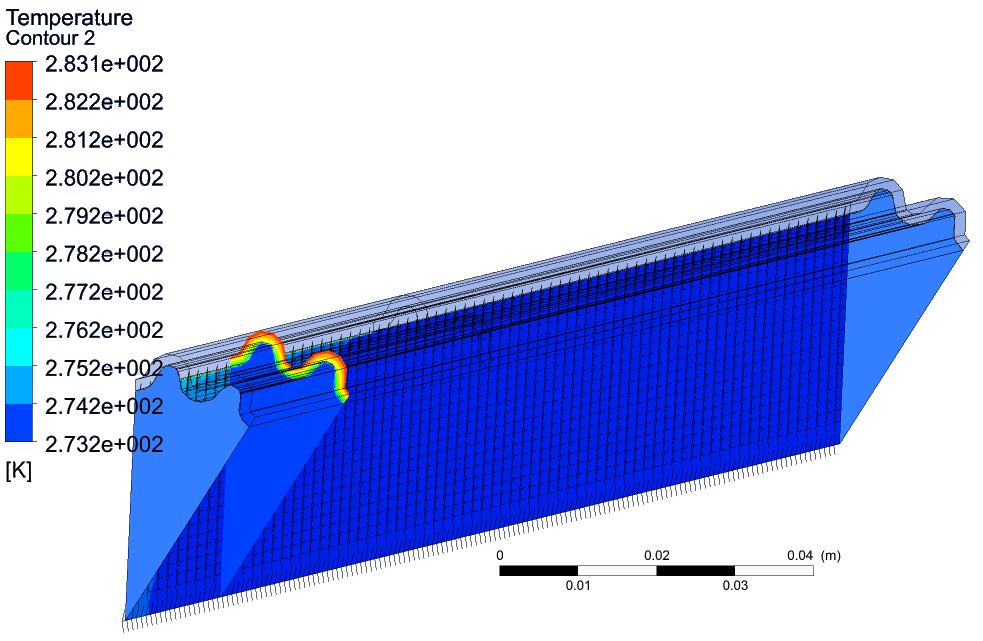
\includegraphics[width=\linewidth]{pipe_nobg}	
	\label{fig:pipe}
\end{subfigure}
\begin{subfigure}{.5\textwidth}
	\centering
	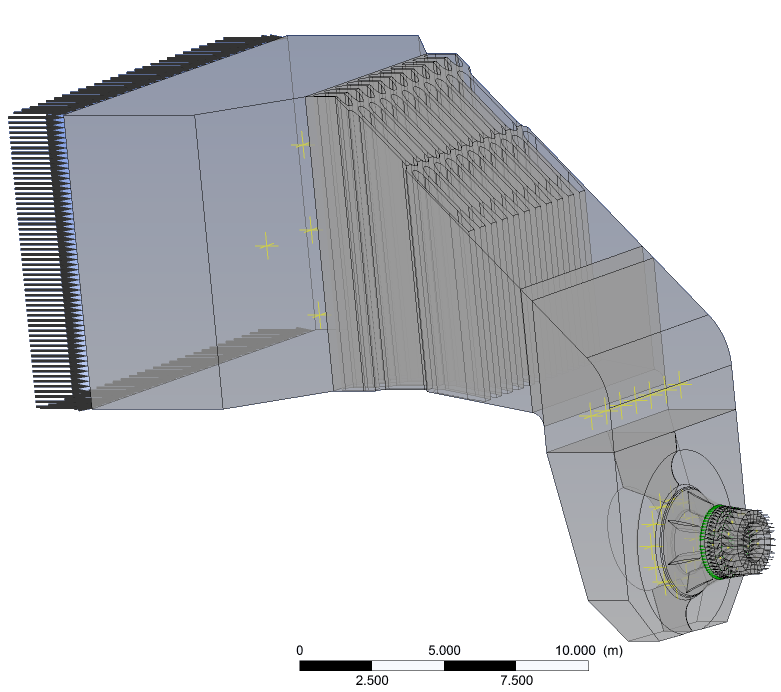
\includegraphics[width=.7\linewidth]{compressor_nobg}
	\label{fig:compressor}
\end{subfigure}

\caption{The geometries of the heat exchange system (left) and compressor (right) used for the simulations. }
\label{fig:cfx}
\end{figure}

To understand the potential scaling impediments on the most powerful Azure nodes, we tested both weak and strong scaling for different simulations cases. With strong scaling, the problem size remains the same, while the number of cores increases, while with the weak scaling, both the problem size and the number of cores increase. These scalability tests provide insights on how fast the same problem can be solved when the number of cores increases, and how to solve a larger problem in the same time. 

% pointed out that there’s another way to scale up a parallel
%program to run on more cores: increase the size of the problem being solved as you increase the number of cores. This is known as weak scaling.


The first scaling defined  provides insights into parallel scalability and memory utilization while the weak scaling approximates the utilization of cores. Since it is difficult to compare different systems, namely a local cluster and the cluster in the cloud and use the Amdahl's Law, from the data available at Figs.~\ref{fig:strongHSR} and \ref{fig:weakPipe} we calculate the speedup $S(N,K)$ as follows: 

\begin{equation}
\label{eq:speedupStrong}
S(N,K) = \frac{T_{seq}(N,1)}{T_{par}(N,K)}
\end{equation}
where the numerator is the running time of the sequential version of the software on a single core, the denominator is the parallel version running on $K$ cores and $N$ is the data size. Ideally the speedup should be equal to $K$. Since this is often not the case, we also calculated the \textit{efficiency of strong scaling} ($E_s(N,K)$), a metric that measures how close to the ideal scaling the speedup actually is (see \ref{kaminsky15} for more details):

$$
E_s(N,K) = S(N,K) / K
$$
 

%Since ANSYS CFX is a commercial software we could not judge what is the sequential and parallizable fraction of the solver. One can only speculate about the that since the performance degrades, the significant 
Sizeup ($S_u$) is a chief metric for measuring the weak scaling. It can be defined as 

\begin{equation}
\label{eq:sizeup}
S_u(N,K) = \frac{N(K)}{N(1)} \times \frac{T_{seq}(N(1),1)}{T_{par}(N(K),K).}
\end{equation}
Because in the weak scaling the problem size is growing as the number of cores increases we denote it as $N(K)$ to emphasize this dependence. Similarly to Eq.~\ref{eq:speedupStrong} $T_{seq}(.)$ denotes the running time of sequential version on a single core. For the scenario where the program's problem size running on K cores is K times larger than the program's problem size running on a single core, the running time for parallel and sequential execution should be the same and the sizeup should be equal to K. The efficiency is the metric that shows how close is the sizeup to the ideal one: 
$$
E_w(N,K) = S_u(N,K) / K
$$
It is equal to 1 no matter on how many cores the program is executed, for worser sizeup values the efficiency is less than 1. It is also worth noting that the sizeup (Eq.~\ref{eq:sizeup}) reduces to speedup $S(N,K)$ (Eq.~\ref{eq:speedupStrong}) because the problem size for the sequential and parallel version are the same and the first fraction in Eq.~\ref{eq:sizeup} becomes unity. Sizeup and speedup measure actually the same entity, e.g. the ratio of computation rates, but in different contexts.

\begin{figure}
\centering
	\centering
	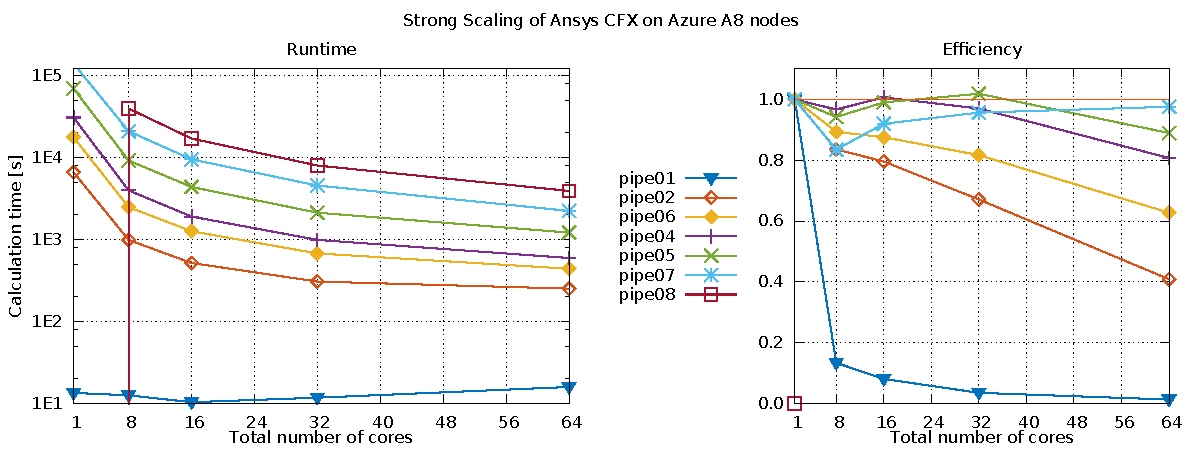
\includegraphics[width=.7\linewidth]{gplt-a8-strong-pipe}	
	\caption{Strong scaling of Ansys CFX Solver on Microsoft Azure A8 nodes. }
	\label{fig:strongA8}
\end{figure}

\begin{figure}
	\centering
	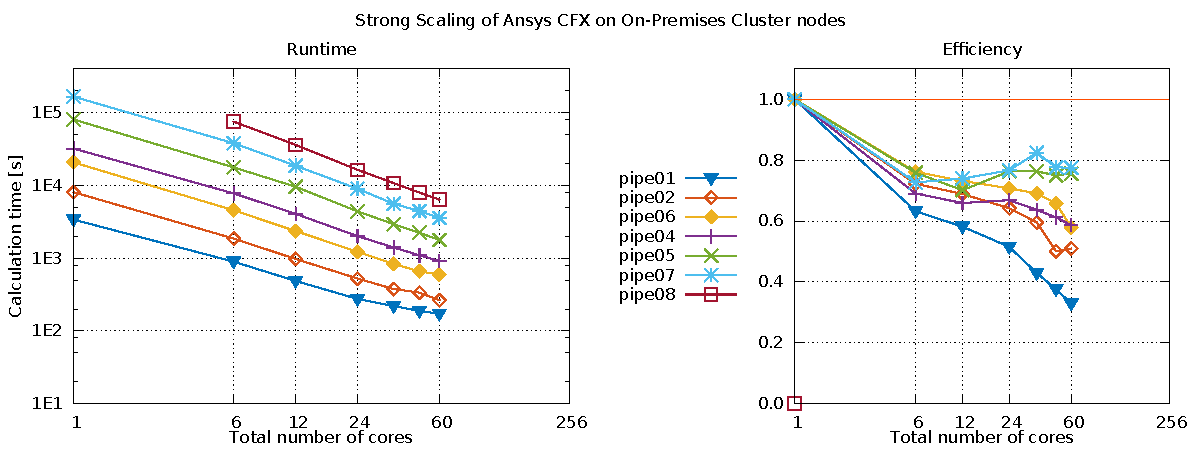
\includegraphics[width=.7\linewidth]{gplt-hsr-strong-pipe}
	\caption{Strong scaling of Ansys CFX Solver on HSR Cluster nodes. }
	\label{fig:strongHSR}
\end{figure}





\begin{figure}
\centering
\begin{subfigure}{.4\textwidth}
	\centering
	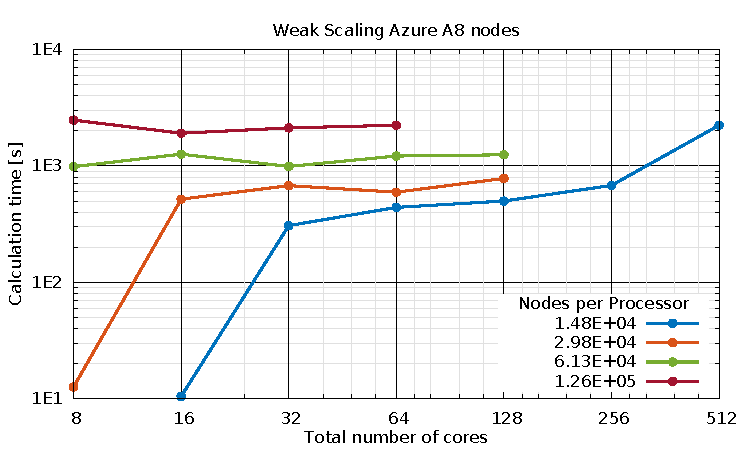
\includegraphics[width=\linewidth]{gplt-a8-weak-pipe}	
	%\label{fig:weakA8}
\end{subfigure}
\begin{subfigure}{.4\textwidth}
	\centering
	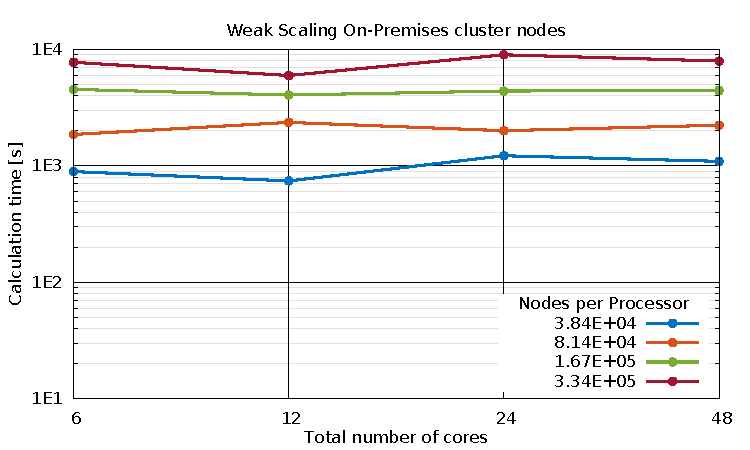
\includegraphics[width=\linewidth]{gplt-hsr-weak-pipe}
	%\label{fig:weakHSR}
\end{subfigure}

\caption{Weak scaling in Microsoft Azure on A8 nodes (left) and HSR cluster (right). }
\label{fig:weakPipe}
\end{figure}

%Todo: Fix caption
\begin{figure}
	\centering
	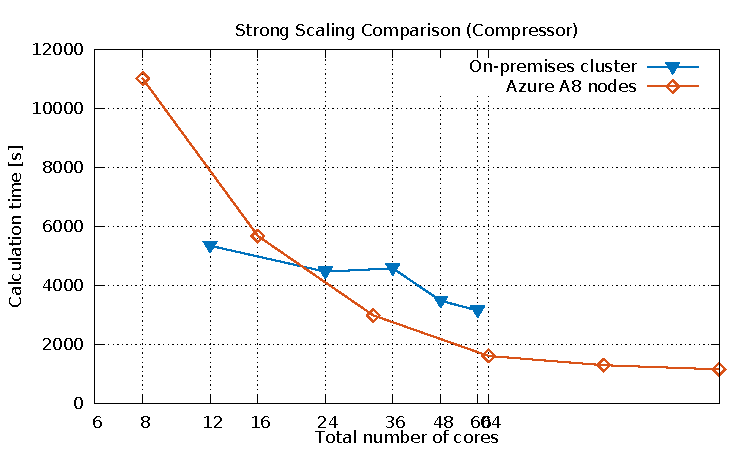
\includegraphics[width=0.5\linewidth]{gplt-compressor}
	\caption{Strong scaling comparison for the compressor geometry). }
	\label{fig:compressor}
\end{figure}


%\subsection{Cost efficiency}
%
%According to the IDC \cite{Perry2007} hardware generates only 7\% of Total Cost of Ownership (TCO) of a cluster operating for three years. Remaining costs are related to staffing, equipment, maintenance, middleware, and training. A yearly cost of a core hour $C_{core/h}$ can be calculated as follows \cite{ubercloud}:
%$$ 
%C_{core/h} = { C_p * T } / { N * 365 * 24 * U } 
%$$
%where $C_p$ is a cost of the cluster, $T$ is a TCO over a year being equal to $7\% * 1/3$ of the cluster cost, $N$ corresponds to the number of cores and $U$ is the average yearly utilization of the cluster. According to this formula $C_{core/h}$ is equal to $0.7\$$ with the average utilization of $30\%$. The price of the HSR cluster was $150k\$$ and according to the above equation, $C_{core/h}$ is $0.71$ for $100\%$ utilization of the system. Since the average utilization of HPC clusters is always much less. e.g. between $20$ and $3	0 \%$ \cite{Delimitrou:2014:QRQ:2541940.2541941} the price raises in more realistic scenarios (see Tab.~\ref{tab:cost}).
%
%\begin{table}[h]
%\begin{tabular}{lccccccccc}
%\hline
%\multicolumn{1}{|l|}{No. of nodes}          & \multicolumn{1}{c|}{1}       & \multicolumn{1}{c|}{2}      & \multicolumn{1}{c|}{3}     & \multicolumn{1}{c|}{8}    & \multicolumn{1}{c|}{10}     & \multicolumn{1}{c|}{12}    & \multicolumn{1}{c|}{16}   & \multicolumn{1}{c|}{24}   & \multicolumn{1}{c|}{32}   \\ \hline
%\multicolumn{1}{|l|}{Utilization {[}\%{]}}  & \multicolumn{1}{c|}{0.03125} & \multicolumn{1}{c|}{0.0625} & \multicolumn{1}{c|}{0.125} & \multicolumn{1}{c|}{0.25} & \multicolumn{1}{c|}{0.3125} & \multicolumn{1}{c|}{0.375} & \multicolumn{1}{c|}{0.5}  & \multicolumn{1}{c|}{0.75} & \multicolumn{1}{c|}{100}  \\ \hline
%\multicolumn{1}{|l|}{$C_{core/h}$ {[}\${]}} & \multicolumn{1}{c|}{22.65}   & \multicolumn{1}{c|}{11.32}  & \multicolumn{1}{c|}{5.66}  & \multicolumn{1}{c|}{2.83} & \multicolumn{1}{c|}{2.26}   & \multicolumn{1}{c|}{1.89}  & \multicolumn{1}{c|}{1.42} & \multicolumn{1}{c|}{0.94} & \multicolumn{1}{c|}{0.71} \\ \hline
                                            %& \multicolumn{1}{l}{}         & \multicolumn{1}{l}{}        & \multicolumn{1}{l}{}       & \multicolumn{1}{l}{}      & \multicolumn{1}{l}{}        & \multicolumn{1}{l}{}       & \multicolumn{1}{l}{}      & \multicolumn{1}{l}{}      & \multicolumn{1}{l}{}     
%\end{tabular}
%\label{tab:cost}
%\caption{Cost of the core per hour for different utilizations of the cluster. }
%\end{table}
%
%These calculations as well the price list in Tab.~\ref{tab:azureVMs} served to compare the cost of a single GFLOP in both systems. This metric was chosen to demonstrate the savings the cloud can bring in terms of performance since this is an important indicator when running numerical simulations (see Fig.\ref{fig:cost}). It turns out that even for less realistic utilization of the private cluster the cost for running in the cloud can be still lower in terms of computing power. For most realistic utilization of $30\%$ When the costs of a single GFLOP are compared directly it turns out the cloud can be much cheaper, especially for large deployment, for example running eight A8 machines can be $19$ times cheaper as on the cluster. Therefore for small organizations a cloud may be an attractive alternative because it eliminates an up-front commitment and provides per-per-use option. SMEs can start small and only scale out when there is a need. 

\section{Conclusion}
\label{sec:conclusions}

We presented SimplyHPC framework, a novel distributed framework for Microsoft Azure Cloud. The framework is composed of light weight modules and a set of commandlets on top of that. The modules automate the complex deployment procedure that is necessary to run third-party applications from the local machine. In contrary to HPC Pack from Microsoft, all unnecessary system components and services have been omitted. As a result the time needed to deploy the cluster has been reduced from nearly an hour to couple of minutes.  This way scientific applications can access the cloud if the calculations are too time-consuming for a local machine or a private cluster. Specially designed mechanism keeps track of running jobs in the cluster. A special service in the head node regularly checks the job status and uploads the results to the blob storage as soon as the job finished successfully. Since a table and blob storage are distributed and mirrored, a high-availability and persistence of the job data is also provided. SimplyHPC software is available at GitHub at https://github.com/vbaros/SimplyHPC.


%Further areas of work could include the following:

\section{Acknowledgments}
\label{sec:ackn}

The framework has been developed in Microsoft Innovation Center in Rapperswil, Switzerland. The scalability tests have been performed in Microsoft Azure as a part of Microsoft Research Grant No. Azdem187T64934Y. We would like also express our gratitude to Adrian Rohner, Roman Fuchs, Rita Rueppel and Vladimir Baros from University of Applied Sciences in Rapperswil for support and fruitful discussions.

\section{Literature}
\label{sec:literature}

\bibliography{hpconAzure}
\bibliographystyle{plain}

\end{document}


